\twocolumn[\colorsection{Fuerza magnética}]
\setcounter{figure}{0}

\begin{Exercise}\label{p:fmagnetica01}
  Un alambre de un metro de largo lleva una corriente $i = \SI{10}{A}$ y forma un ángulo de $\SI{30}{\degree}$ con un campo magnético uniforme de módulo $B = \SI{1.5}{\tesla}$, como indica la figura \ref{f:fmagnetica01}. Calcular la fuerza que actúa sobre el alambre.
\end{Exercise}
\begin{Answer}
  $\va*{F} = \SI{7.5}{\newton}\vu{z}$
\end{Answer}
%
\begin{center}
  \begin{tikzpicture}[scale=0.5]
    \draw (6,0) ellipse (0.1 and 0.2);
    \draw (-5,0) +(90:0.1 and 0.2) arc (90:270:0.1 and 0.2);
    \draw [black] (-5,0.2)--(6,0.2);
    \draw [black] (-5,-0.2)--(6,-0.2);
    \draw [blue, -{Stealth}] (-6,-2.7)--(-3,-2.7) node[black,right,right] {$x$};
    \draw [blue, -{Stealth}] (-5,-3)--(-5,-1) node[black,above,left] {$y$};
    \draw [red, -{Stealth}] (-4.33,-2.5)--(4.33,2.5) node[black,above,above left] {$\va*{B}$};
    \draw [red, -{Stealth}, thick] (-4,0)--(-1,0) node[black,midway,above left] {$i$};
    \draw [red, -{Stealth}] (-6,-0.577)--(-0.66,2.5);
    \draw [red] (0.66,-2.5)--(6,0.577);
    \draw[-latex] (0:3.5) arc (0:30:3.5) node[black,midway,right] {$30^\circ$};
  \end{tikzpicture}
  \captionof{figure}{Problema \ref{p:fmagnetica01}\label{f:fmagnetica01}}
\end{center}
%
\begin{Exercise}\label{p:fmagnetica02}
  La figura \ref{f:fmagnetica02} muestra una bobina rectangular suspendida del brazo de una balanza analítica. Pende entre los polos de un electroimán con el plano de la bobina paralela a las caras de los polos. En la región marcada el campo magnético es uniforme y es despreciablemente pequeño en las proximidades de la parte superior del hilo. La bobina tiene 15 vueltas y la longitud del lado de la base es de $\SI{8}{\centi\metre}$. Cuando circula una corriente igual a $\SI{0.4}{\ampere}$ por la bobina debemos añadir una sobrecarga de $\SI{60.5}{\gram}$ al platillo de la derecha para establecer el equilibrio en el sistema. Determinar cuál el módulo del campo magnético.
\end{Exercise}
\begin{Answer}
  $\SI{1.24}{\tesla}$
\end{Answer}
%
\begin{center}
  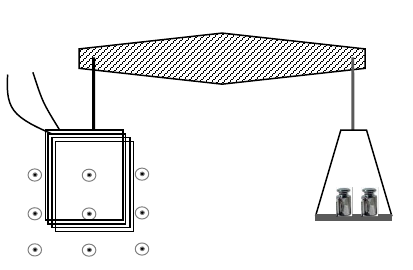
\includegraphics[scale=0.6]{m02.png}
  \captionof{figure}{Problema \ref{p:fmagnetica02}\label{f:fmagnetica02}}
\end{center}
%
\begin{Exercise}\label{p:fmagnetica03}
  La figura \ref{f:fmagnetica03} muestra una bobina con 20 espiras cuadradas, de lado igual $\SI{5}{\centi\metre}$, por la que circula la corriente $i = \SI{0.10}{\ampere}$. Verificar que el momento sobre una espira puede calcularse como $\va*{M} = \va*{m} \times \va*{B}$, donde $\va*{m}$ es el momento magnético de la espira, y hallar qué momento actúa sobre la bobina si está colocada de forma que el plano forma un ángulo $\alpha = \SI{60}{\degree}$ con respecto al eje $i$, en presencia de un campo magnético uniforme $\va*{B} = \SI{0.50}{\tesla}\vu{j}$.
\end{Exercise}
\begin{Answer}
  $\va*{M} = \SI{-2.17E-3}{\newton . \metre}\vu{k}$
\end{Answer}
%
\begin{center}
  \tdplotsetmaincoords{70}{120}
  \begin{tikzpicture}[tdplot_main_coords, scale=0.7]
    \draw[axis] (0,0,0) -- (4,0,0) node [pos=1.1] {$i$};
    \draw[axis] (0,0,0) -- (0,4,0) node [pos=1.05] {$j$};
    \draw[axis] (0,0,0) -- (0,0,4)  node [left] {$k$};
    \draw[] (0,0,0) -- (2,3,0) -- (2,3,3) -- (0,0,3) -- cycle;
    \draw[] (0.1,-0.05,0) -- (2.1,2.95,0) -- (2.1,2.95,3) -- (0.1,-0.05,3) -- cycle;
    \draw[] (-0.1,0.05,0) -- (1.9,3.05,0) -- (1.9,3.05,3) -- (-0.1,0.05,3) -- cycle;
    \draw[red, -{latex}, very thick] (0.2,0,1) -- (0.2,0,2.5) node [midway, left] {$i$};
    \draw[red, -{latex}, thick] (0.9,-2.5,1.25) -- (0.9,-0.5,1.25);
    \draw[red, -{latex}, thick] (0.9,3,1.25) -- (0.9,5,1.25) node [midway, above] {$\va*{B}$};
    \draw[red, -{latex}, thick] (0.9,-2.5,2.5) -- (0.9,-0.5,2.5);
    \draw[red, -{latex}, thick] (0.9,3,2.5) -- (0.9,5,2.5);
    \draw[red, -{latex}, thick] (0.9,-2.5,0) -- (0.9,-0.5,0);
    \draw[red, -{latex}, thick] (0.9,3,0) -- (0.9,5,0);
    \draw[-latex] (0:2.5) arc (0:53:2.5) node[black,midway,below] {$\alpha$};
  \end{tikzpicture}
  \captionof{figure}{Problema \ref{p:fmagnetica03}\label{f:fmagnetica03}}
\end{center}
%
\begin{Exercise}\label{p:fmagnetica04}
  Una barra conductora tiene $\SI{40}{\centi\metre}$ de longitud y $\SI{30}{\gram}$ de masa, y desliza libremente sobre las tiras metálicas de los extremos del plano inclinado mostrado en la figura \ref{f:fmagnetica04}, conectadas entre sí por un segmento conductor en la base de la rampa, mientras una corriente $i$ fluye a través del circuito indicado. El ángulo del plano inclinado es $\alpha = \SI{37}{\degree}$ y el sistema está inmerso en un campo magnético uniforme $\va*{B} = \SI{-0.20}{\tesla}\vu{y}$. ¿De qué magnitud debe ser $i$ para que la barra permanezca en reposo?
\end{Exercise}
\begin{Answer}
  $\SI{2.77}{\ampere}$
\end{Answer}
%
\begin{center}
  \tdplotsetmaincoords{50}{110}
  \begin{tikzpicture}[tdplot_main_coords, scale=0.7]
    \draw[axis] (0,0,0) -- (4.5,0,0) node [pos=1.1] {$z$};
    \draw[axis] (0,0,0) -- (0,7,0) node [pos=1.05] {$x$};
    \draw[axis] (0,0,0) -- (0,0,3)  node [left] {$y$};
    \filldraw[draw=black,fill=black!50!green!50] (0,0,0) -- (0,6,3) -- (0.2,6,3) -- (0.2,0,0) -- cycle;
    \filldraw[draw=black, fill=black!50!green!50] (3,0,0) -- (3,6,3) -- (3.2,6,3) -- (3.2,0,0) -- cycle;
    \filldraw[draw=black, fill=black!50!green!50] (0,0,0) -- (3.2,0,0) -- (3.2,-0.2,0) -- (0,-0.2,0) -- cycle;
    \filldraw[draw=black, fill=red!30] (3.2,4,2) -- (3.2,4.402,2.201) -- (3.2,4.301, 2.402) -- (3.2, 3.9, 2.201) -- cycle;
    \filldraw[draw=black, fill=red!40] (3.2,3.9,2.201) -- (3.2,4.301,2.402) -- (0,4.301,2.403) -- (0,3.9,2.201) -- cycle;
    \filldraw[draw=black, fill=red!60] (3.2,4.301,2.402) -- (0,4.301,2.402) -- (0,4.402,2.201,2.402) -- (3.2,4.402,2.201,2.402) -- cycle;
    \draw[dotted] (3.1,0,0) -- (3.1,6,0);
    \draw[dotted] (0,6,0) -- (0,6,3) -- (3.1,6,3) -- (3.1,6,0) -- cycle;
    \draw[red, -{latex}, thick] (2.5,-0.3,0) -- (0.5,-0.3,0) node [midway, left] {$i$};
    \draw[red, -{latex}, thick] (-0.2,1,0.5) -- (-0.2,3,1.5) node [midway, above] {$i$};
    \draw[red, -{latex}, thick] (3.4,3,1.5) -- (3.4,1,0.5) node [midway, below] {$i$};
    \tdplotdrawarc{(3.1,1,0)}{2.5}{90}{136}{right}{$\alpha$}
  \end{tikzpicture}
  \captionof{figure}{Problema \ref{p:fmagnetica04}\label{f:fmagnetica04}}
\end{center}
%
\begin{Exercise}\label{p:fmagnetica05}
  Un conductor que transporta una corriente $i = \SI{3.0}{\ampere}$, está doblado sobre el plano $xy$ como se muestra en la figura \ref{f:fmagnetica05} y permanece en una zona donde existe un campo magnético $\va*{B} = \SI{0.70}{\tesla}\vu{x}$. El radio $R$ del semicírculo es $\SI{0.50}{\metre}$. ¿A qué fuerza está sometido el conductor?
\end{Exercise}
\begin{Answer}
  $\va*{F} = \SI{-2.1}{\newton}\vu{z}$
\end{Answer}
%
\begin{center}
  \begin{tikzpicture}[scale=0.5]
    \draw (5,0) ellipse (0.05 and 0.1);
    \draw [black] (0,0.1)--(5,0.1);
    \draw [black] (0,-0.1)--(5,-0.1);
    \draw [black] (0,0.1) arc (270:90:3);
    \draw [black] (0,-0.1) arc (270:90:3.2);
    \draw (5,6.2) ellipse (0.05 and 0.1);
    \draw [black] (0,6.1)--(5,6.1);
    \draw [black] (0,6.3)--(5,6.3);
    \draw [red, -{Stealth}, thick] (1,5.8)--(3,5.8) node[midway,below] {$i$};
    \draw [red, -{Stealth}, thick] (3,0.5)--(1,0.5) node[midway,above] {$i$};
    \draw [red, -{Stealth}, thick] (-1.84,1.26) arc (225:180:2.6) node[midway,right] {$i$};
    \draw [blue, -{Stealth}] (1,2)--(3,2) node[black,right,right] {$x$};
    \draw [blue, -{Stealth}] (1.3,1.7)--(1.3,3.7) node[black,above,left] {$y$};
    \draw [dotted] (0,0.1)--(0,6.1);
    \draw [dashed] (0,3.1)--(-2.12,5.22) node[midway,above] {$R$};
    \draw [blue, -{Stealth}] (-6,3.1)--(-4,3.1) node[pos=-0.2] {$\va*{B}$};
    \draw [blue, -{Stealth}] (-6,2.1)--(-4,2.1);
    \draw [blue, -{Stealth}] (-6,1.1)--(-4,1.1);
    \draw [blue, -{Stealth}] (-6,0.1)--(-4,0.1);
    \draw [blue, -{Stealth}] (-6,4.1)--(-4,4.1);
    \draw [blue, -{Stealth}] (-6,5.1)--(-4,5.1);
    \draw [blue, -{Stealth}] (-6,6.1)--(-4,6.1);
  \end{tikzpicture}
  \captionof{figure}{Problema \ref{p:fmagnetica05}\label{f:fmagnetica05}}
\end{center}
%
\begin{Exercise}\label{p:fmagnetica06}
  Mostrar que para la espira de la figura \ref{f:fmagnetica06}, por la cual circula una corriente y se encuentra sumergida en un campo magnético uniforme perpendicular al plano de la espira, la fuerza resultante es nula.
\end{Exercise}
%
\begin{center}
  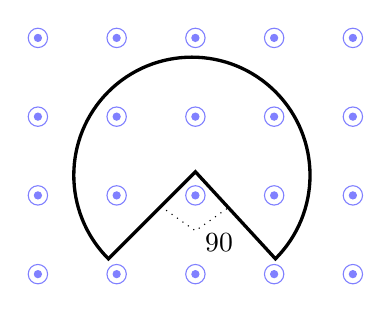
\begin{tikzpicture}[scale=0.5]
    \draw [very thick] (-2.21,0.79) arc (225:-45:3) -- (0,3) -- cycle;
    \draw [dotted] (-0.88,2.12) -- (0,1.5) -- (0.88,2.12);
    \draw (0,1.2) node [right] {$\SI{90}{\degree}$};
    \def\a{-4};
    \def\b{0.4};
    \def\d{2};
    \foreach \x in {0,...,4}
    \foreach \y [count=\yi] in {0,...,3}
    {
      \fill [blue!100!black!50] (\a+\d*\x,\b+\d*\y) circle (3pt);
      \draw [blue!100!black!50] (\a+\d*\x,\b+\d*\y) circle (7pt);
    }
  \end{tikzpicture}
  \captionof{figure}{Problema \ref{p:fmagnetica06}\label{f:fmagnetica06}}
\end{center}
%
\begin{Exercise}
  Un electrón se está moviendo con una velocidad de $\SI{4E6}{\metre/\second}$ en la dirección positiva del eje $x$, cuando ingresa en una zona del espacio donde existe un campo eléctrico uniforme $\va*{E} = \SI{2000}{\volt/\metre}\vu{y}$. Encontrar el campo magnético necesario para que en esa región el electrón no se desvíe de su trayectoria.
\end{Exercise}
\begin{Answer}
  $\va*{B} = \SI{5E-4}{\tesla}\vu{z}$
\end{Answer}
%
\begin{Exercise}\label{p:fmagnetica07}
  Un electrón pasa por el punto $A$ de la figura \ref{f:fmagnetica07} con una velocidad de módulo $V_0 = \SI{1E7}{\metre/\second}$. Calcular: \textit{a}) El valor y el sentido del campo magnético uniforme que obliga al electrón a seguir la trayectoria semicircular desde $A$ hacia $B$. \textit{b}) El tiempo necesario para que el electrón se mueva desde $A$ hasta $B$.
\end{Exercise}
\begin{Answer}
  \begin{minipage}[t]{.4\textwidth}
    \textit{a}) $\SI{1.138E-3}{\tesla}$, perpendicular y entrando a la hoja\\ \textit{b}) $\SI{1.57E-8}{\second}$
  \end{minipage}
\end{Answer}
%
\begin{center}
  \begin{tikzpicture}[scale=0.5]
    \draw [blue, -{Stealth}] (0,0) -- (0,3) node [left] {$V_0$};
    \draw [dashed] (0,0) arc (180:0:5);
    \draw [dotted] (0,0) -- (10,0);
    \draw [{Stealth}-{Stealth}] (0,-0.5) -- (10,-0.5) node[midway,below] {$\SI{10}{\centi\metre}$};
    \draw [] (0,-0.3) -- (0,-0.8);
    \draw [] (10,-0.3) -- (10,-0.8);
    \draw (0,0) node [left] {$A$};
    \draw (10,0) node [right] {$B$};
  \end{tikzpicture}
  \captionof{figure}{Problema \ref{p:fmagnetica07}\label{f:fmagnetica07}}
\end{center}
%
\begin{Exercise}\label{p:fmagnetica08}
  Un ion que parte del reposo en el vacío es acelerado por dos placas paralelas entre las que existe una ddp de $\SI{1000}{\volt}$ como indica la figura \ref{f:fmagnetica08}. Al salir de la segunda placa, el ion se mueve bajo la acción de un campo magnético uniforme de módulo $B = \SI{0.1}{\tesla}$, normal al plano de la trayectoria. Si el radio de curvatura de la trayectoria es $\SI{0.3}{\metre}$, ¿cuál es la masa del ion si su carga es la del electrón?
\end{Exercise}
\begin{Answer}
  $\SI{7.2E-26}{\kilogram}$
\end{Answer}
%
\begin{center}
  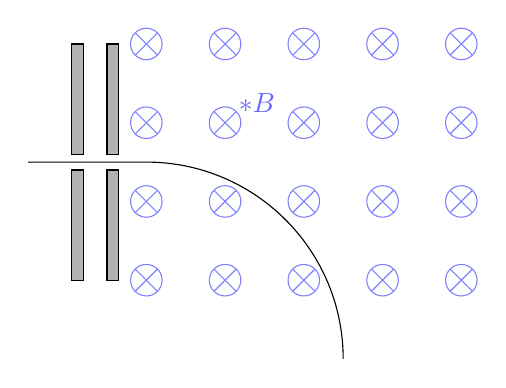
\begin{tikzpicture}[scale=0.5]
    \draw [] (-7,3.4) -- (-4,3.4) arc (90:0:5) ;
    \draw [blue!100!black!60] (-1.9,4.4) node[above right] {$\va*{B}$};
    \filldraw [draw=black, fill=black!30] (-5,0.4) -- (-5,3.2) -- (-4.7,3.2) -- (-4.7,0.4) -- cycle;
    \filldraw [draw=black, fill=black!30] (-5,3.6) -- (-5,6.4) -- (-4.7,6.4) -- (-4.7,3.6) -- cycle;
    \filldraw [draw=black, fill=black!30] (-5.9,0.4) -- (-5.9,3.2) -- (-5.6,3.2) -- (-5.6,0.4) -- cycle;
    \filldraw [draw=black, fill=black!30] (-5.9,3.6) -- (-5.9,6.4) -- (-5.6,6.4) -- (-5.6,3.6) -- cycle;
    \def\a{-4};
    \def\b{0.4};
    \def\d{2};
    \foreach \x in {0,...,4}
    \foreach \y [count=\yi] in {0,...,3}
    {
      % \fill [blue!100!black!50] (\a+\d*\x,\b+\d*\y) circle (3pt);
      \draw [blue!100!black!50] (\a+\d*\x-0.2828,\b+\d*\y-0.2828) -- (\a+\d*\x+0.2828,\b+\d*\y+0.2828);
      \draw [blue!100!black!50] (\a+\d*\x+0.2828,\b+\d*\y-0.2828) -- (\a+\d*\x-0.2828,\b+\d*\y+0.2828);
      \draw [blue!100!black!50] (\a+\d*\x,\b+\d*\y) circle (0.4);
    }
  \end{tikzpicture}
  \captionof{figure}{Problema \ref{p:fmagnetica08}\label{f:fmagnetica08}}
\end{center}
%
\begin{Exercise}
  Un electrón con una energía de $\SI{2.0}{keV}$ se dispara en un campo uniforme de $\SI{0.10}{\tesla}$ y su velocidad forma un ángulo de $\SI{89}{\degree}$ con el mismo. Muestre que la trayectoria será una hélice, con su eje en la dirección del campo. Encuentre el periodo $T$, el paso $p$ y el radio $r$ de la hélice.
\end{Exercise}
\begin{Answer}
  \begin{minipage}[t]{.4\textwidth}
    $T=\SI{3.57E-10}{\second}$\\ $p=\SI{0.16}{\milli\metre}$\\ $r=\SI{1.5}{\milli\metre}$
  \end{minipage}
\end{Answer}

